\chapter{Experimental setup and methodology}
\section{Introduction}
In this chapter, the aim of the experiment, the experimental procedure, the materials, the analysis of samples, and the detailed experimental methods employed are all concisely described. The analysis of the methods and the testing standards utilized are presented. These include the microstructural analysis, environmental stress cracking tests, and corrosion analysis of the three materials of interest, which are mild steel, stainless steel, and HDPE. All the parameters used are discussed and shown with the safety precautions being followed throughout the experiments. After AFFF solution has been exposed to various engineering materials, the composition and other vital performance parameters are critically analyzed.

\section{Aim of the experiment}
The experimental work aims to evaluate and assess the impact and compatibility of the storage facility (engineering materials) on the composition of AFFF, hence performance parameters. 

\section{Methodology}
Samples of stainless-steel, mild steel, and HDPE together with AFFF solution were carefully prepared. A guillotine machine was used to cut the material sheets into desired shapes and sizes. All the material sheets were cut to the same sizes and shapes for a fair comparison. A total of 5 samples were used during the experiments. These sample materials were exposed to natural environmental conditions, with another sample of mild steel being exposed to seawater for 60 days. All the samples were then immersed and soaked in 3\% proportion of AFFF solution for further 120 days. Fourier transform infrared spectroscopy (FTIR), Transmission electron microscopy (TEM), Dynamic Light Scattering (DLS), and Inductively Coupled Plasma (ICP) wet analysis were performed on sample materials. This was done to analyse the composition, properties and stability of AFFF solution after being exposed to these materials. 
During the tests, clean sample materials and AFFF solution from the manufacturer were used as a benchmark and their properties were compared to the exposed material to deduce any vital changes occurred. All the findings were carefully recorded and analysed. However, it should be noted that the objective was to analyze the AFFF solution. The experimental procedure followed for all the samples is presented in the flowchart in Figure \ref{ch4:figure:procedure}. 

\begin{figure}[H]
\centering

\begin{tikzpicture}[node distance=3cm]
    \tikzstyle{block} = [rectangle, minimum height=1.5cm, inner sep=1em, text centered, text width=5cm, draw=black]
    \tikzstyle{arrow} = [thick, ->, >=stealth]

    \node (prepare) [block] {Prepared materials and AFFF solution samples};

    \node (expose) [block, below of=prepare] {Exposed material samples to natural environmental conditions 60 days};

    \node (immerse) [block, below of=expose] {Immersed and soaked material samples to AFFF solution for 5 months};

    \node (perform) [block, right of=prepare, xshift=6cm] {Performed FTIR, TEM, DLS and ICP tests on material samples};

    \node (test) [block, below of=perform] {Tested and analysed the elementary composition and performance parameters on AFFF solution};

    \node (analyse) [block, below of=test] {Data analysis};

    \newcommand*{\connector}[4][]{
        \draw[#1] (#3) -| ($(#3) !#2! (#4)$) |- (#4);
    }

    \draw [arrow] (prepare) -- (expose);
    \draw [arrow] (expose) -- (immerse);

    \connector[->, black]{0.5}{immerse}{perform}

    \draw [arrow] (test) -- (analyse);

\end{tikzpicture}

\caption{Typical experimental procedure}
\label{ch4:figure:procedure}
\end{figure}

\section{Material description}
On the present experiments, 3, 4 and 5mm sheets of duplex stainless steel, mild steel and HDPE respectively were selected as the materials of interest. The sample sheets were scribed to ease and ensure that the cut sizes are precise during the cutting stage. The cut samples were further cut to three small pieces for accurate testing and the average results were considered. This was also done to accommodate the percentage errors and external factors which may have occurred during the experimental setup. Glass beakers of 800ml in volume were prepared to fill the 3\% proportion of AFFF solution and immerse the material samples. 

\section{Sample preparation}
\subsection{Experimental matrix}

\begin{table}[H]

\centering
\begin{tabular}{m{.25\textwidth} m{.25\textwidth} m{.4\textwidth}}
    \hline
    Material & Instrument & Analyses \\
    \hline
    AFFF solution & FTIR & Functional groups \\
    & TEM & Particle size and shape \\
    & & HR imaging \\
    & & Electron diffraction images \\
    & DLS & Particle size distribution \\
    & ICP & Elementary identification \\
    \hline
\end{tabular}

\caption{Experimental matrix with AFFF solution.}
\end{table}

\subsection{Material plates} 
The sheets of stainless steel, mild steel, and HDPE respectively were prepared for the experiments. These sheets required to be cut to the desired shapes and sizes so that they can fit in beakers filled with AFFF solution. The scriber was used to scribe the precise sizes and the shapes to be cut. This was done at the Durban University of Technology (DUT) manufacturing workshop, using a guillotine cutting machine. The prepared material samples can be seen in Figure \ref{ch4:figure:stainless_steel}, \ref{ch4:figure:mild_steel} and \ref{ch4:figure:hdpe}.
 
\begin{figure}[H]
    \centering
    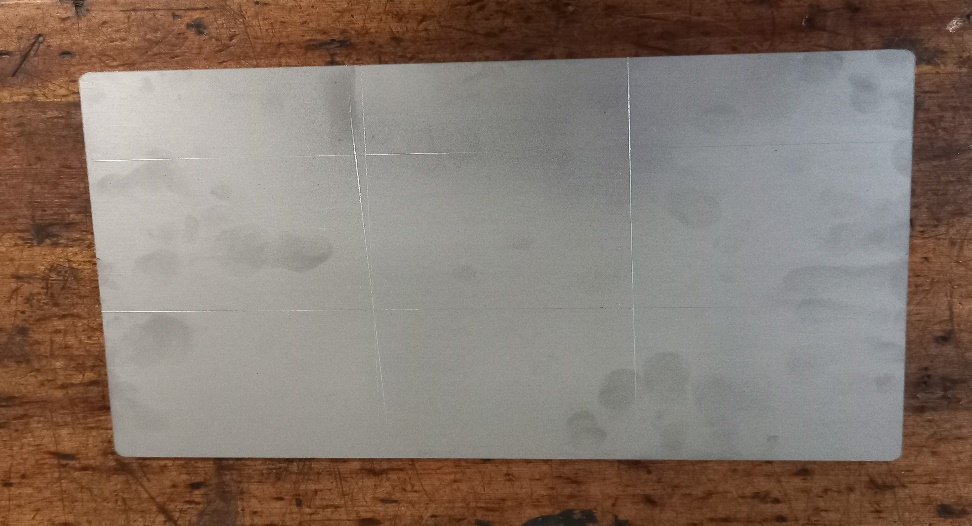
\includegraphics[width=.55\textwidth]{duplex_stainless_steel_sample.jpg}
    \caption{Duplex stainless steel sample.}
    \label{ch4:figure:stainless_steel}
\end{figure}
 
\begin{figure}[H]
    \centering
    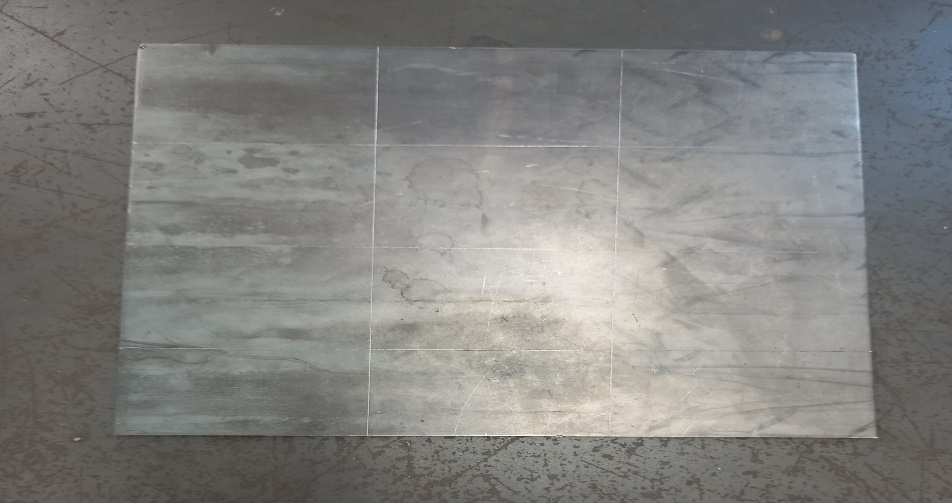
\includegraphics[width=.55\textwidth]{mild_steel_sample.jpg}
    \caption{Mild steel sample.}
    \label{ch4:figure:mild_steel}
\end{figure}

\begin{figure}[H]
    \centering
    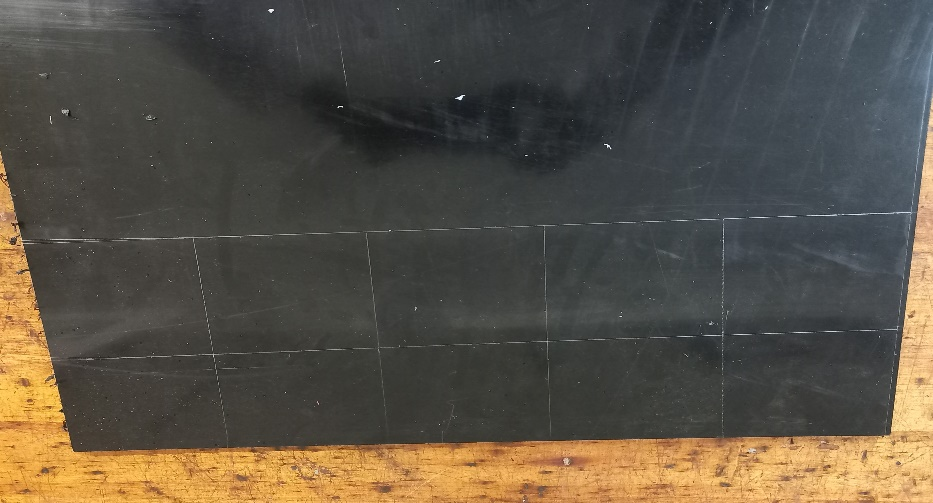
\includegraphics[width=.55\textwidth]{hdpe_sample.jpg}
    \caption{HDPE sample}
    \label{ch4:figure:hdpe}
\end{figure}

\subsection{The cutting process}
The prepared samples were cut to the sizes of 60mm x 100mm using a guillotine machine. It can be seen in Figures \ref{ch4:figure:stainless_steel}, \ref{ch4:figure:mild_steel} and \ref{ch4:figure:hdpe} that the samples were firstly scribed before being cut to ensure the precision. Stainless steel and mild steel were cut using a guillotine that can cut up to a thickness of 5mm. In contrast HDPE was cut in guillotine that can cut up to 3mm thickness, it is not hard as the two steels. Figure \ref{ch4:figure:5mm_guillotine} and \ref{ch4:figure:3mm_guillotine} shows the two guillotine machines that were used to cut the samples.
 
\begin{figure}[H]
    \centering
    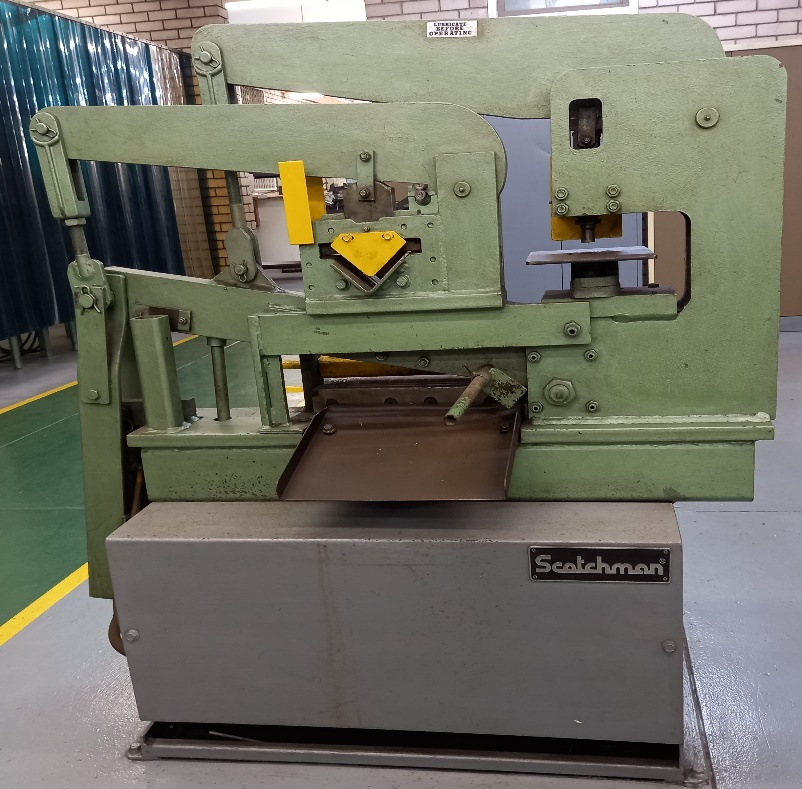
\includegraphics[width=.4\textwidth]{5mm_guillootine_machine.jpg}
    \caption{Guillotine machine that cuts up to 5mm thickness.}
    \label{ch4:figure:5mm_guillotine}
\end{figure}
 
\begin{figure}[H]
    \centering
    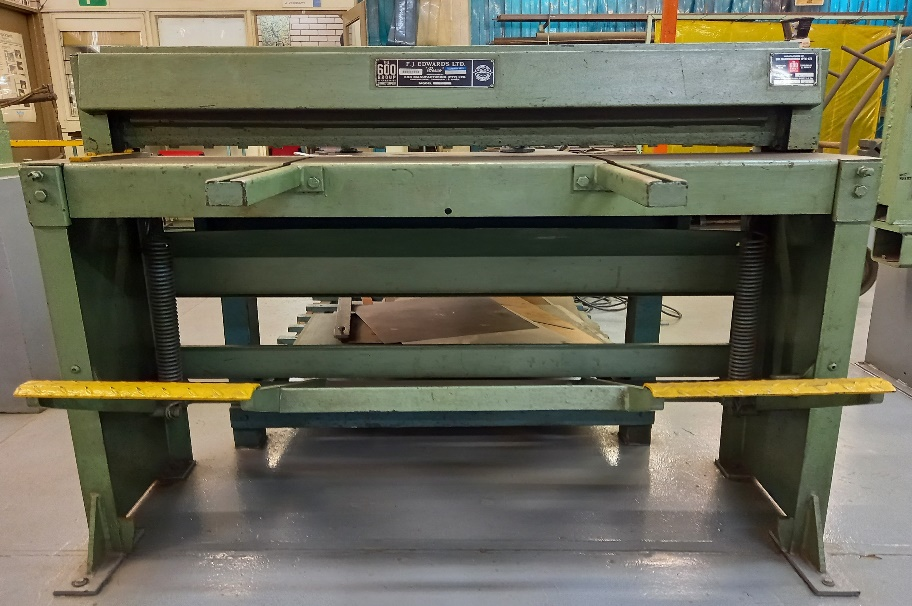
\includegraphics[width=.55\textwidth]{3mm_guillotine_machine.jpg}
    \caption{Guillotine machine that cuts up to 3mm thickness}
    \label{ch4:figure:3mm_guillotine}
\end{figure}

As indicated in section 4.5.3 the samples were cut to numerous pieces and to the desired shapes and size to fit glass beakers. Figure \ref{ch4:figure:samples} shows the samples after the cutting process. 
 
\begin{figure}[H]
    \centering
    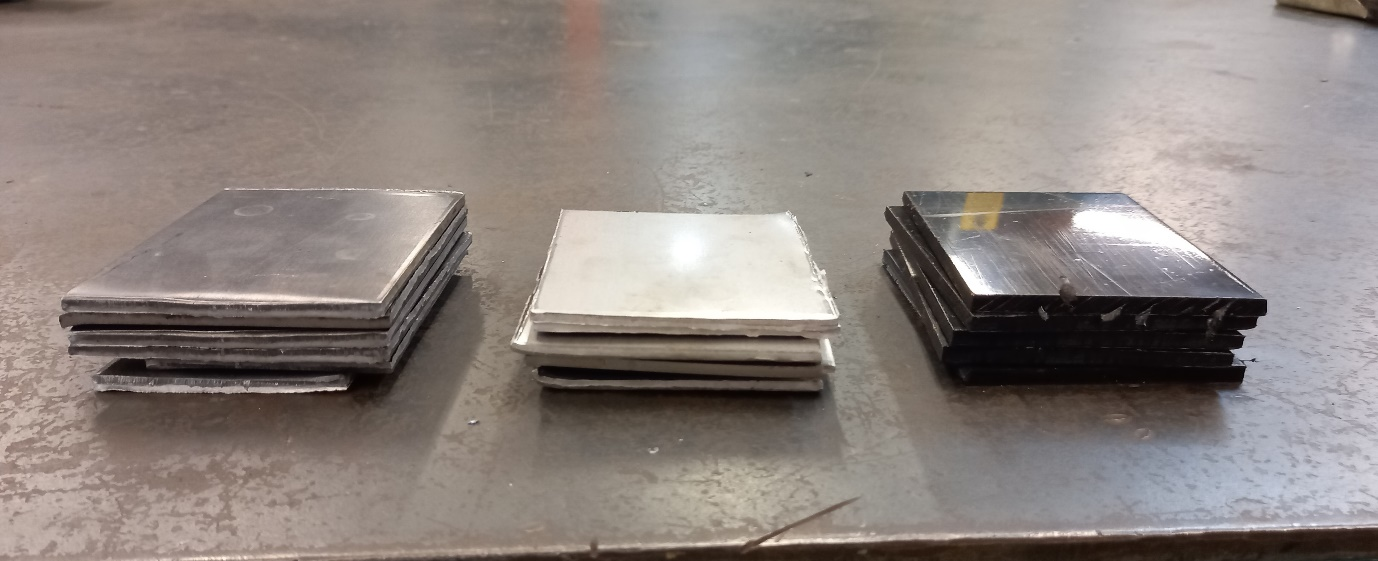
\includegraphics[width=.8\textwidth]{samples_after_being_cut.jpg}
    \caption{Samples after being cut to the desired sizes.}
    \label{ch4:figure:samples}
\end{figure}

The samples were polished and cleaned using the rectangular file. This was done to remove the roughness and dangerous chips, to avoid any possible injuries during the experimental setup. Figure \ref{ch4:figure:file_and_vice} shows the tools used when cleaning and polishing the samples.
 
\begin{figure}[H]
    \centering
    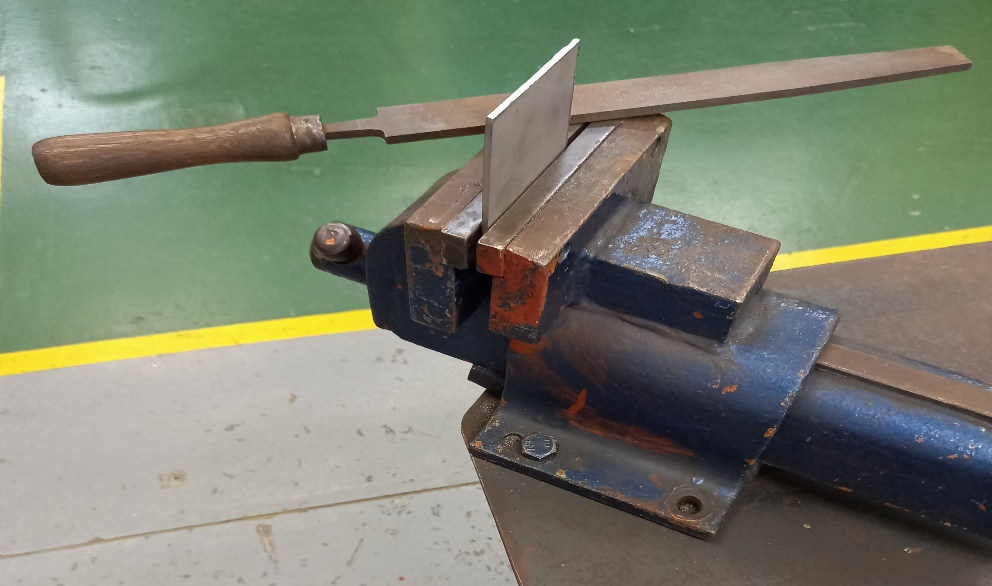
\includegraphics[width=.6\textwidth]{rectangular_file_and_bench_vice.jpg}
    \caption{Rectangular file and bench vice}
    \label{ch4:figure:file_and_vice}
\end{figure}

\subsection{AFFF solution samples}
The 3\% proportion AFFF solution samples were prepared in 20 litres each and stored in room temperature at the laboratory in DUT. These were carefully stored in their original containers until the material samples were available and ready. Figure \ref{ch4:figure:mild_steel} shows the AFFF solution from the suppliers in 20 litre containers.
Picture of AFFF 20 litres
AFFF solution were filled in respective glass beakers to immerse various material samples. There were 10 glass beakers which were prepared in total. Only four beakers were used initially, with the first 2 glass beakers being prepared for clean HDPE that was immersed in AFFF solutions to investigate whether the solution will initiate the ESC on HDPE. The other two beakers were filled with seawater and then mild steel was immersed to increase the rate of corrosion. Figure \ref{ch4:figure:hdpe_immersed} shows the first 4 glass beakers used during the experimental work.
 
\begin{figure}[H]
    \centering
    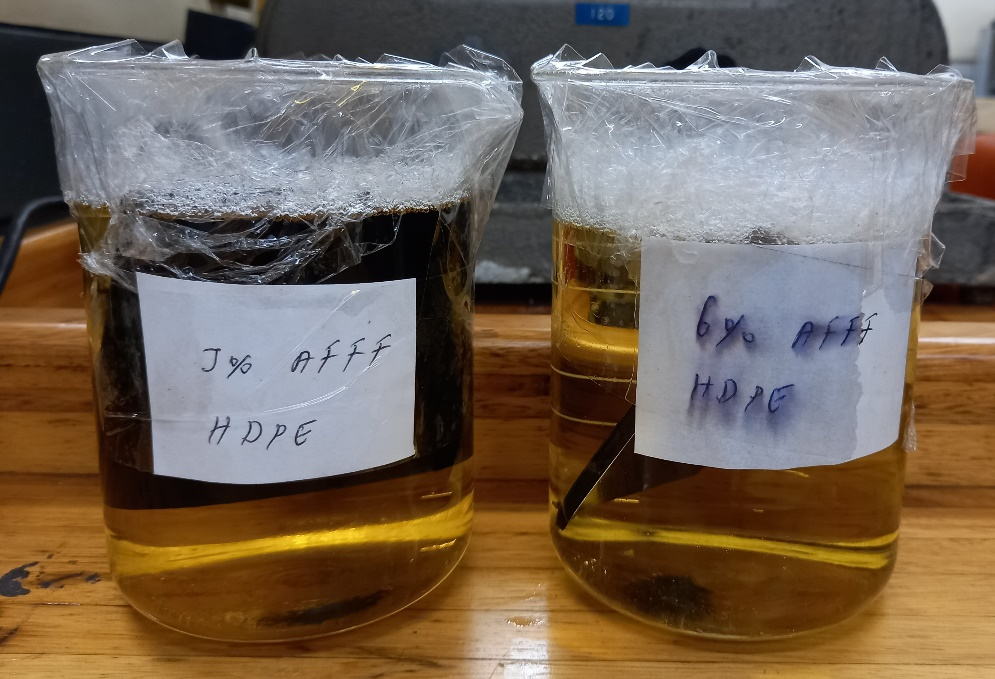
\includegraphics[width=.5\textwidth]{hdpe_immersed_in_various_afff_solutions.jpg}
    \caption{HDPE immersed in various AFFF solutions.}
    \label{ch4:figure:hdpe_immersed}
\end{figure}
 
\begin{figure}[H]
\centering
\begin{subfigure}{\textwidth}
    \centering
    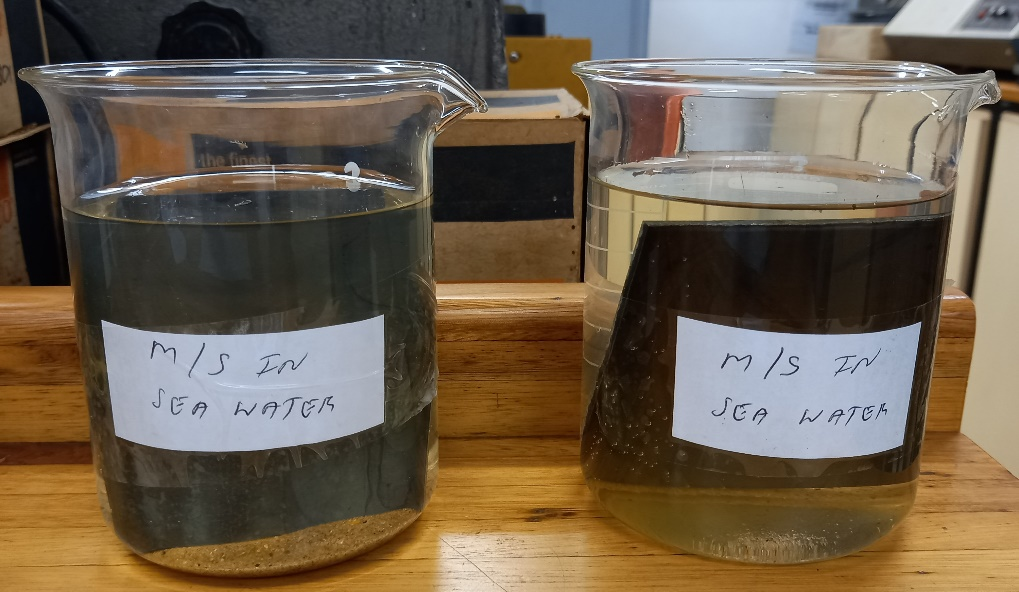
\includegraphics[width=.5\textwidth]{mild_steel_immersed_in_seawater.jpg}
\end{subfigure}
\par\medskip
\begin{subfigure}{\textwidth}
    \centering
    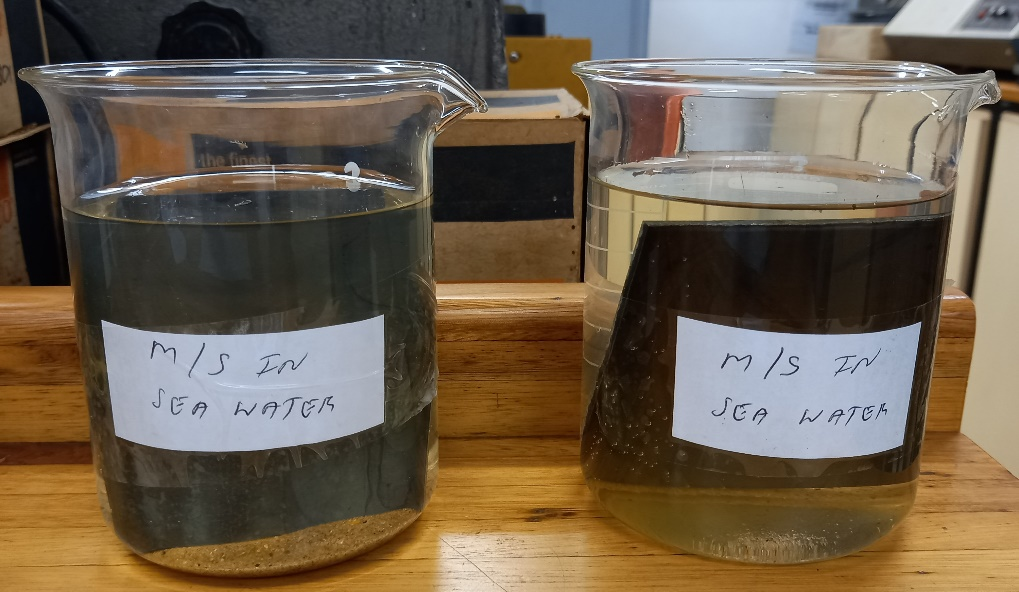
\includegraphics[width=.5\textwidth]{mild_steel_immersed_in_seawater.jpg}
\end{subfigure}

\caption{Mild steel immersed in seawater.}
\label{ch4:figure:steel_immersed}
\end{figure}

\section{Testing} 
The different tests that were performed after the experiments are discussed in this section. The apparatus and various materials that were utilised when conducting the tests are concisely described. 
Fourier transform infrared spectroscopy (FTIR), Transmission electron microscopy (TEM), Dynamic Light Scattering and Inductively Coupled Plasma (ICP)

\subsection{Fourier transform infrared spectroscopy (FTIR)}
All the AFFF samples were analyzed using the FTIR technique. This was achieved by comparing the clean samples that were from the manufacturer with the samples that has been exposed to various materials experiments. The FTIR analysis assisted in identifying the functional groups for various exposed samples.
 
\begin{figure}[H]
    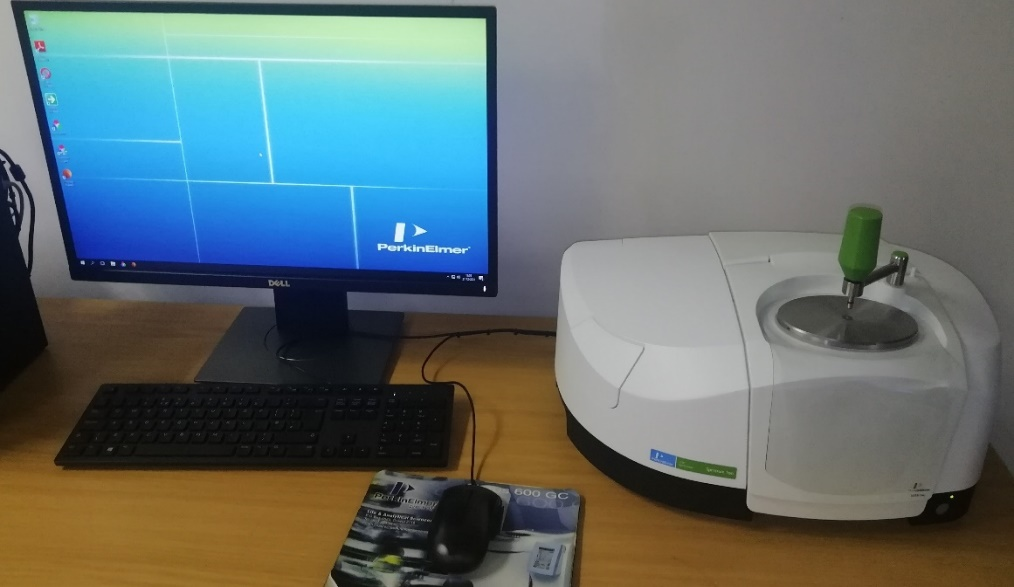
\includegraphics[width=.6\textwidth]{ftir_instrument.jpg}
    \caption{FTIR instrument used for functional groups.}
    \label{ch4:figure:ftir}
\end{figure}

\subsection{Transmission electron microscopy (TEM)}
Since the FTIR does not provide conclusive information, it was essential to validate the FTIR analysis with other tests. TEM analysis were conducted to analyse large variety of particle, overall particle shape, and visual overall size and shape of the AFFF solution particles using HR imaging and electron diffraction images. It should be noted that TEM does not provide sufficient information on how the particles in the exposed AFFF solution are distributed and does not covey the precise particle sizes. 
 
\begin{figure}[H]
    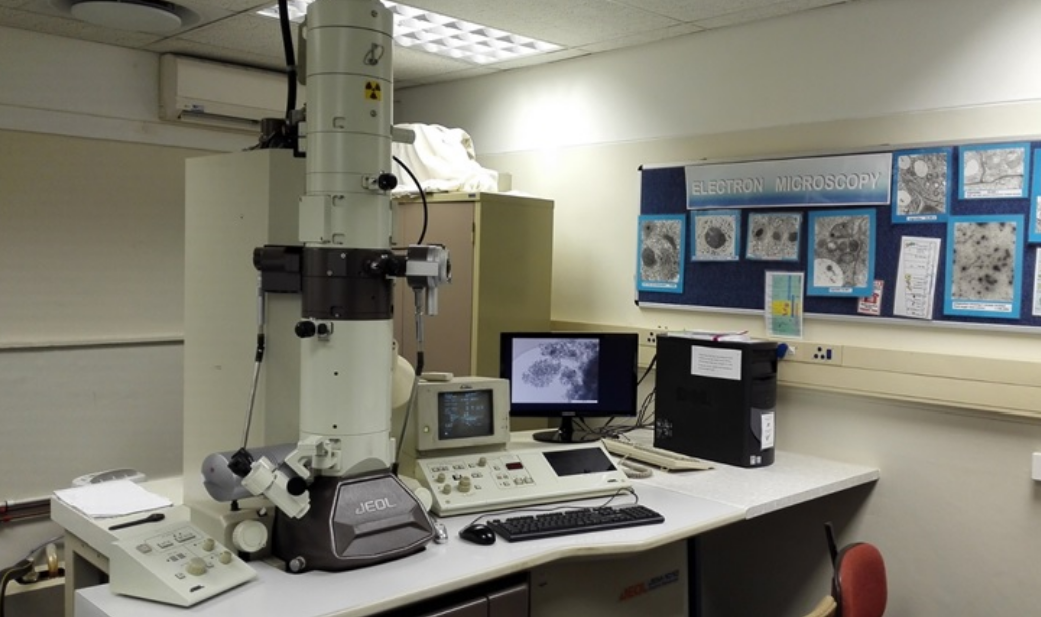
\includegraphics[width=.6\textwidth]{tem_instrument.png}
    \caption{TEM instrument used to analyze particles.}
    \label{ch4:figure:tem}
\end{figure}

\subsection{Dynamic Light Scattering (DLS)}
The DLS tests were conducted to deduce the particle size distribution and precise particle sizes. This was achieved by measurement of the hydrodynamic diameter (Z-average) of any present particles in units of nm. This was done to validate the findings of TEM, and it further assisted in depth understanding of the behaviour of the AFFF solution particles when exposed to various materials and how they affect its properties.  
 
\begin{figure}[H]
    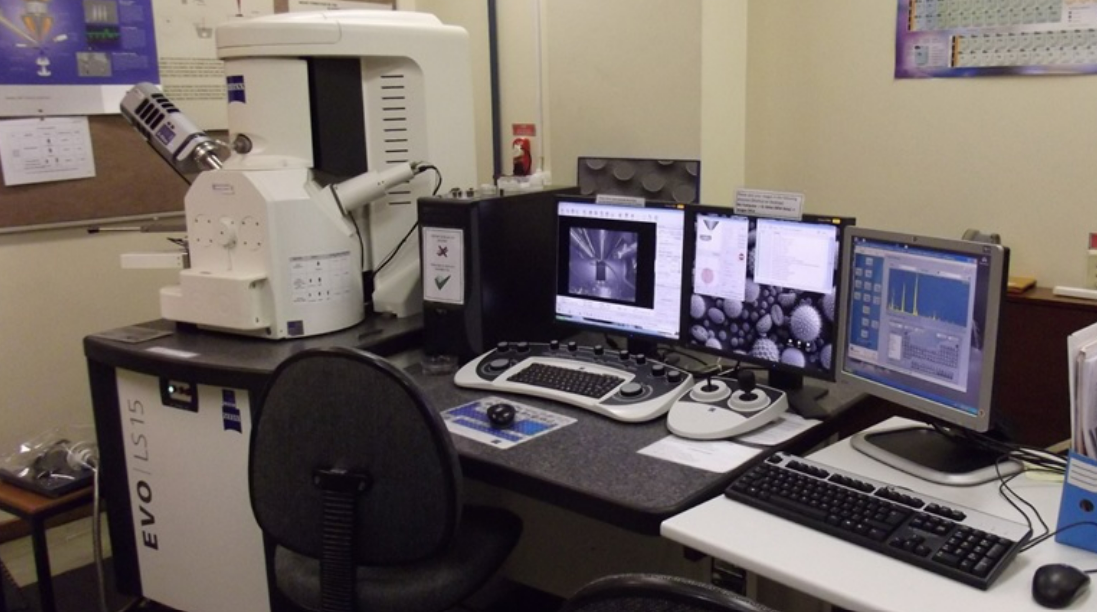
\includegraphics[width=.6\textwidth]{dls_instrument.png}
    \caption{DLS instrument used to analyze particle distribution.}
    \label{ch4:figure:dls}
\end{figure}

\subsection{Inductively Coupled Plasma (ICP)}
Finally, the ICP test was conducted to identify the chemical elements or composition within the exposed AFFF solution and benchmark these with the standard qualities. The changes in chemical composition can greatly affect the properties, hence the performance of AFFF during the firefighting circumstances. Thus, it is vital to assess the impact of the various materials on the composition of the AFFF solution. 
 
\begin{figure}[H]
    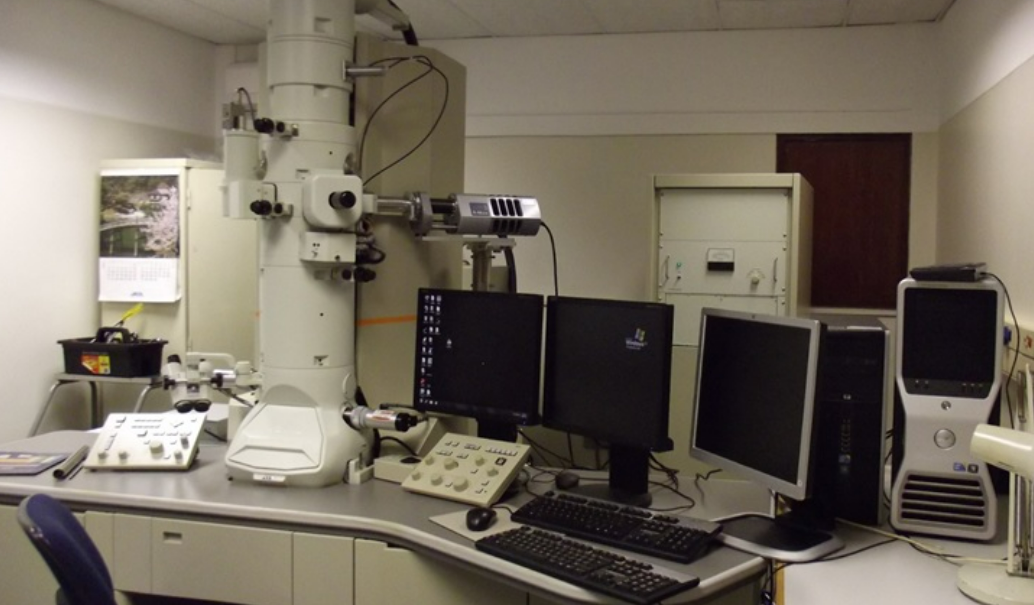
\includegraphics[width=.6\textwidth]{icp_instrument.png}
    \caption{ICP instrument used for elementary analysis.}
    \label{ch4:figure:icp}
\end{figure}

\section{Summary}
The present chapter outlined the aim of the experiment, the material description, sample preparation, the techniques employed to test the samples and as well as the equipment and testing standards used. The instruments used for analysing the AFFF solution samples were presented with thorough explanation of the purpose of each test. The experimental procedure followed in this investigation was explained. The results from the investigation are presented in chapter 5.